\section{Binary Search Trees}

\subsection{Binary Trees}

A \textbf{tree} is a hierarchical data structure made of \textbf{nodes} connected by edges/pointers.  
Unlike arrays or linked lists, trees do not store data linearly. Instead, they branch.

Each node contains:
\begin{itemize}
  \item a value
  \item a reference to a left child (optional)
  \item a reference to a right child (optional)
\end{itemize}

\textbf{Binary trees} restrict each node to at most two children.

\textbf{Tree terminology:}
\begin{itemize}
  \item \textbf{Root}: the topmost node
  \item \textbf{Parent}: a node that points to children
  \item \textbf{Child}: a node pointed to by a parent
  \item \textbf{Leaf}: a node with no children
  \item \textbf{Depth}: number of edges from the root to a node
  \item \textbf{Height}: number of edges in the longest path from a node to a leaf
\end{itemize}

\subsection{Binary Search Trees}

A \textbf{Binary Search Tree (BST)} is a binary tree with a \textbf{sorted property}:

\begin{itemize}
  \item For \textbf{every node}, all values in its left subtree are \textbf{less than} the node's value
  \item For \textbf{every node}, all values in its right subtree are \textbf{greater than} the node's value
\end{itemize}

This property makes a BST behave like a sorted array, allowing us to eliminate half of the tree at every step during search. 

Assuming that a BST is perfectly balanced, searching, inserting and deleting are all $O(\log n)$ operations. Meanwhile, arrays require $O(n)$ shifts for insert/delete.

\begin{center}
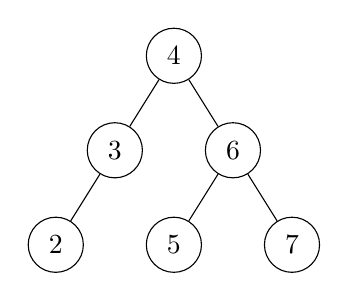
\begin{tikzpicture}[
  level distance=1.2cm,
  every node/.style={circle, draw, minimum size=7mm},
  edge from parent/.style={draw,-}
]
\node {4}
  child { node {3}
    child { node {2} }
    child[missing] {}
  }
  child { node {6}
    child { node {5} }
    child { node {7} }
  };
\end{tikzpicture}
\end{center}

\subsection{BST Search (Recursive)}

Searching in a balanced BST has a time complexity of \textbf{$O(\log n)$} while searching in a unbalanced tree is $O(n)$ as it's essentially been degenerated into a linked list.

\textbf{Example: search for 5}

\begin{center}
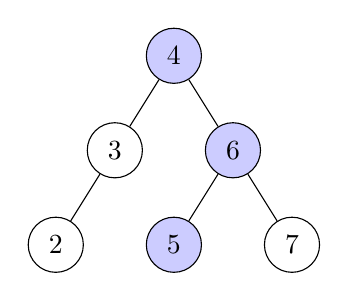
\begin{tikzpicture}[
  level distance=1.2cm,
  every node/.style={circle, draw, minimum size=7mm},
  edge from parent/.style={draw,-},
  highlight/.style={circle, draw, fill=blue!20}
]
\node[highlight] {4}
  child { node {3}
    child { node {2} }
    child[missing] {}
  }
  child { node[highlight] {6}
    child { node[highlight] {5} }
    child { node {7} }
  };
\end{tikzpicture}
\end{center}

Path: $4 \rightarrow 6 \rightarrow 5$

\begin{verbatim}
boolean search(TreeNode root, int target) {
    if (root == null) return false;
    if (root.val == target) return true;
    if (target < root.val) return search(root.left, target);
    else return search(root.right, target);
}
\end{verbatim}

\subsection{Insertion in a BST}

Insertion follows the same logic as search:
\begin{itemize}
  \item If value is smaller, go left
  \item If value is larger, go right
  \item Insert when you hit a null pointer
\end{itemize}

\textbf{Example: insert 1}

\begin{center}
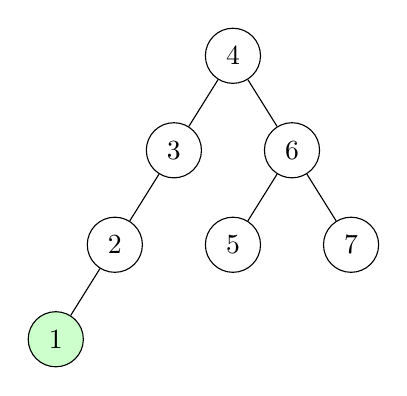
\begin{tikzpicture}[
  level distance=1.2cm,
  every node/.style={circle, draw, minimum size=7mm},
  edge from parent/.style={draw,-},
  new/.style={circle, draw, fill=green!20}
]
\node {4}
  child { node {3}
    child { node {2}
      child { node[new] {1} }
      child[missing] {}
    }
    child[missing] {}
  }
  child { node {6}
    child { node {5} }
    child { node {7} }
  };
\end{tikzpicture}
\end{center}

\begin{verbatim}
TreeNode insert(TreeNode root, int val) {
    if (root == null) return new TreeNode(val);
    if (val < root.val)
        root.left = insert(root.left, val);
    else
        root.right = insert(root.right, val);
    return root;
}
\end{verbatim}

\subsection{Finding the Minimum Value}

The minimum value in a BST is found by going left until we cannot go further.

\begin{center}
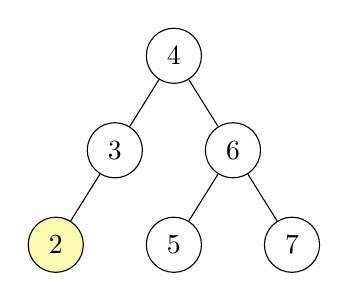
\begin{tikzpicture}[
  level distance=1.2cm,
  every node/.style={circle, draw, minimum size=7mm},
  edge from parent/.style={draw,-},
  highlight/.style={circle, draw, fill=yellow!30}
]
\node {4}
  child { node {3}
    child { node[highlight] {2} }
    child[missing] {}
  }
  child { node {6}
    child { node {5} }
    child { node {7} }
  };
\end{tikzpicture}
\end{center}

\begin{verbatim}
TreeNode findMin(TreeNode root) {
    while (root.left != null)
        root = root.left;
    return root;
}
\end{verbatim}
\subsection{Deleting a Node in a BST}

We use the same example tree throughout:

\begin{center}
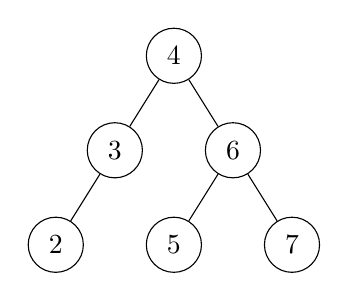
\begin{tikzpicture}[
  level distance=1.2cm,
  every node/.style={circle, draw, minimum size=7mm},
  edge from parent/.style={draw,-}
]
\node {4}
  child { node {3}
    child { node {2} }
    child[missing] {}
  }
  child { node {6}
    child { node {5} }
    child { node {7} }
  };
\end{tikzpicture}
\end{center}

\textbf{Case 1: Leaf node (no children)}  

Example: delete node 2

\begin{center}
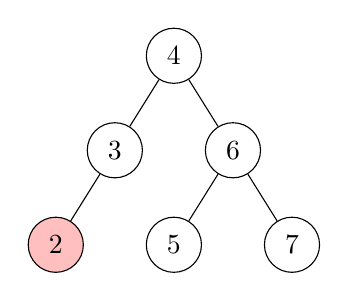
\begin{tikzpicture}[
  level distance=1.2cm,
  every node/.style={circle, draw, minimum size=7mm},
  edge from parent/.style={draw,-},
  removed/.style={circle, draw, fill=red!25}
]
\node {4}
  child { node {3}
    child { node[removed] {2} }
    child[missing] {}
  }
  child { node {6}
    child { node {5} }
    child { node {7} }
  };
\end{tikzpicture}
\end{center}

Node 2 is simply removed and replaced with \texttt{null}.

\bigskip

\textbf{Case 2: Node with one child}  

Example: delete node 3

Return the non-null child.

\begin{center}
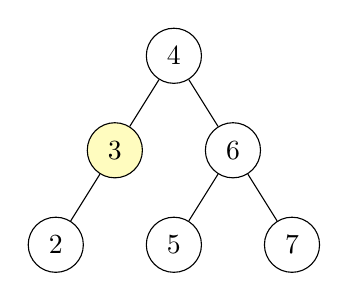
\begin{tikzpicture}[
  level distance=1.2cm,
  every node/.style={circle, draw, minimum size=7mm},
  edge from parent/.style={draw,-},
  highlight/.style={circle, draw, fill=yellow!25}
]



\node {4}
  child { node[highlight] {3}
    child { node {2} }
    child[missing] {}
  }
  child { node {6}
    child { node {5} }
    child { node {7} }
  };
\end{tikzpicture}
\end{center}

After deletion, node 2 moves up to replace node 3.

\bigskip

\textbf{Case 3: Node with two children}  

\textbf{Example: delete node 4}

Replace the node to remove with the smallest leaf node in the right subtree or the largest leaf node in the left subtree. Then delete that leaf.


\textbf{Step 1: find successor}

\begin{center}
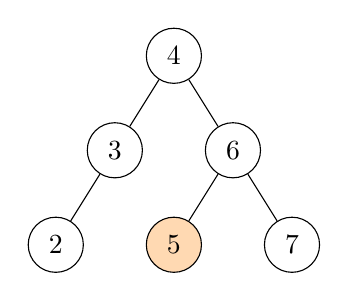
\begin{tikzpicture}[
  level distance=1.2cm,
  every node/.style={circle, draw, minimum size=7mm},
  edge from parent/.style={draw,-},
  highlight/.style={circle, draw, fill=orange!30}
]
\node {4}
  child { node {3}
    child { node {2} }
    child[missing] {}
  }
  child { node {6}
    child { node[highlight] {5} }
    child { node {7} }
  };
\end{tikzpicture}
\end{center}

\textbf{Step 2: replace and delete leaf}

\begin{center}
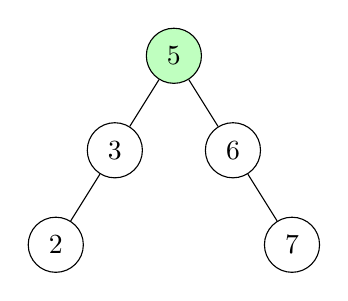
\begin{tikzpicture}[
  level distance=1.2cm,
  every node/.style={circle, draw, minimum size=7mm},
  edge from parent/.style={draw,-},
  newroot/.style={circle, draw, fill=green!25}
]
\node[newroot] {5}
  child { node {3}
    child { node {2} }
    child[missing] {}
  }
  child { node {6}
    child[missing] {}
    child { node {7} }
  };
\end{tikzpicture}
\end{center}

\begin{verbatim}
TreeNode deleteNode(TreeNode root, int key) {
    if (root == null) return null;
    if (key < root.val)
        root.left = deleteNode(root.left, key);
    else if (key > root.val)
        root.right = deleteNode(root.right, key);
    else {
        if (root.left == null) return root.right;
        if (root.right == null) return root.left;
        TreeNode minNode = findMin(root.right);
        root.val = minNode.val;
        root.right = deleteNode(root.right, minNode.val);
    }
    return root;
}
\end{verbatim}


\subsection{Depth-First Search (DFS)}

Depth-first search explores a tree by going as deep as possible before backtracking.  
All traversals below use the following tree:

\begin{center}
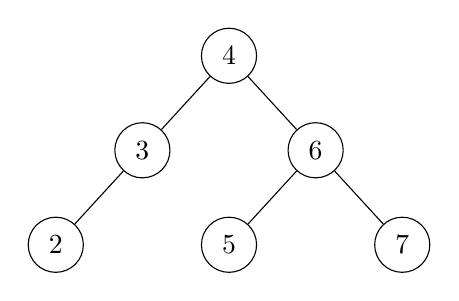
\begin{tikzpicture}[
  level distance=1.2cm,
  sibling distance=2.2cm,
  every node/.style={circle, draw, minimum size=7mm},
  edge from parent/.style={draw,-}
]
\node {4}
  child { node {3}
    child { node {2} }
    child[missing] {}
  }
  child { node {6}
    child { node {5} }
    child { node {7} }
  };
\end{tikzpicture}
\end{center}

There are three common DFS traversal orders:

\textbf{Inorder (left $\rightarrow$ root $\rightarrow$ right)}  
Prints values in sorted order for a BST:
\[
2, 3, 4, 5, 6, 7
\]

\begin{verbatim}
void inorder(TreeNode root) {
    if (root == null) return;
    inorder(root.left);
    System.out.print(root.val + " ");
    inorder(root.right);
}
\end{verbatim}

\textbf{Preorder (root $\rightarrow$ left $\rightarrow$ right)}  
Processes the root before its subtrees (useful for copying/serialization):
\[
4, 3, 2, 6, 5, 7
\]

\begin{verbatim}
void preorder(TreeNode root) {
    if (root == null) return;
    System.out.print(root.val + " ");
    preorder(root.left);
    preorder(root.right);
}
\end{verbatim}

\textbf{Postorder (left $\rightarrow$ right $\rightarrow$ root)}  
Processes children before the parent (useful for deletion/evaluation):
\[
2, 3, 5, 7, 6, 4
\]

\begin{verbatim}
void postorder(TreeNode root) {
    if (root == null) return;
    postorder(root.left);
    postorder(root.right);
    System.out.print(root.val + " ");
}
\end{verbatim}

\subsection{Breadth-First Search (BFS)}

Breadth-first search visits nodes \textbf{level by level}, from top to bottom and left to right.

Using the same tree, BFS prints:
\[
4 \rightarrow 3,6 \rightarrow 2,5,7
\]

BFS uses a \textbf{queue (FIFO)} because nodes are processed in the order they are discovered.

\begin{verbatim}
void bfs(TreeNode root) {
    if (root == null){
        return;
    }

    Queue<TreeNode> q = new LinkedList<>();
    q.add(root);

    while (!q.isEmpty()) {
        TreeNode curr = q.peek();
        System.out.print(curr.val + " ");
        q.remove();

        if (curr.left != null) q.add(curr.left);
        if (curr.right != null) q.add(curr.right);
    }
}
\end{verbatim}

\textbf{Time Complexity:} $O(n)$  
Each node is visited exactly once.